\clearpage
\section{Hybrid defect cavity}

The last geometry simulated is a hybrid cavity with a defect in the centre. The goal is to have the benefits of both the defect cavity, \textit{i.e.} the tunability of the cavity, and hybrid cavity, \textit{i.e.} high purity of output modes. The cavity design is shown in figure \ref{fig:hybrid_defect}.

Figure \ref{fig:hybrid_defect:analysis} shows an analysis of the cavity laser action for a defect of $\frac{\pi}{2}$. As expected this geometry presents the features of both defect and hybrid cavities. Mode 1 in figure \ref{fig:hybrid_defect:intensity} presents strong confinement within the defect while the hybrid structure ensures fairly pure circular polarisation output : the worst polarisation is mode 1 with $\epsilon=37^\circ$.

\begin{figure}
	\centering
	\begin{subfigure}{0.48\linewidth}
		\begin{subfigure}{\linewidth}
			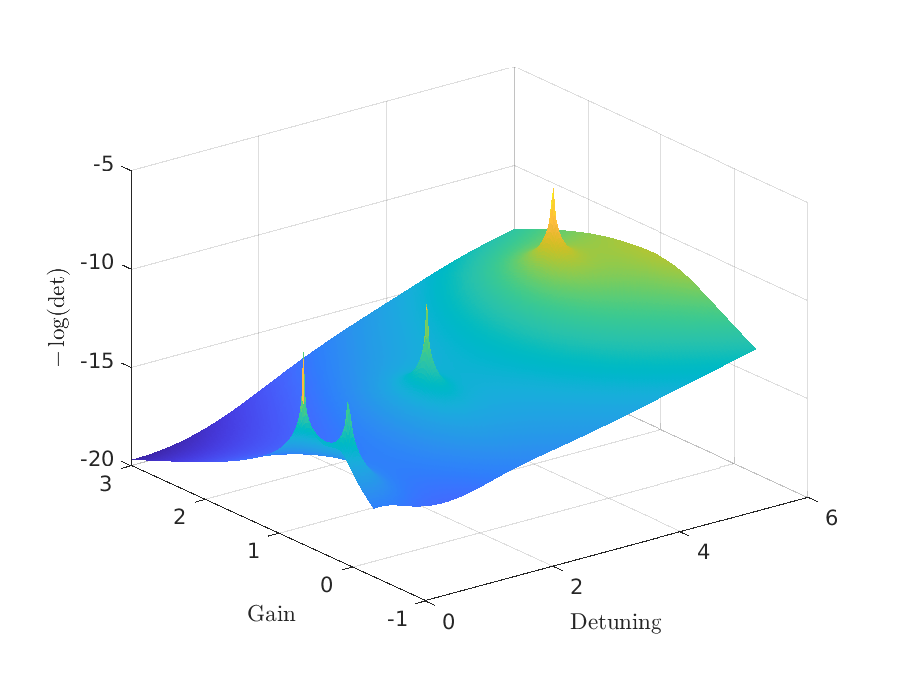
\includegraphics[width=\linewidth]{plots/hybrid_defect/pi_2/surface}
			\caption{}
			\label{fig:hybrid_defect:surf}
		\end{subfigure}
		\begin{subfigure}{\linewidth}
			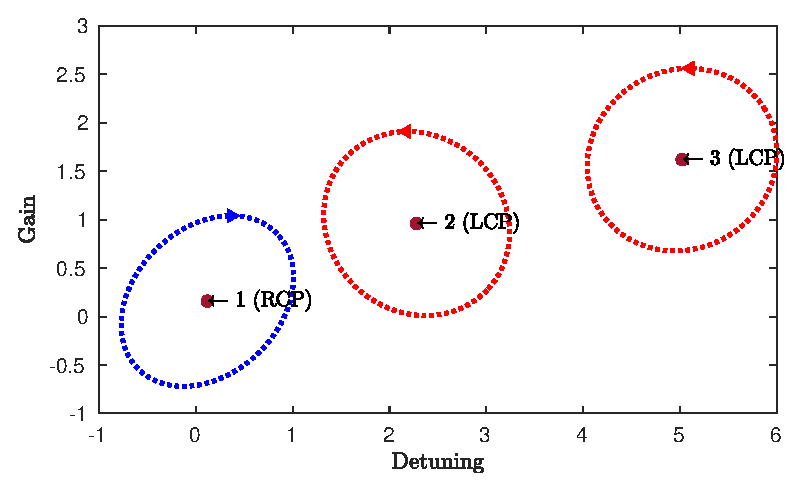
\includegraphics[width=\linewidth]{plots/hybrid_defect/pi_2/modes_found}
			\caption{}
			\label{fig:hybrid_defect:modes}
		\end{subfigure}
	\end{subfigure}
	\begin{subfigure}{0.48\linewidth}
		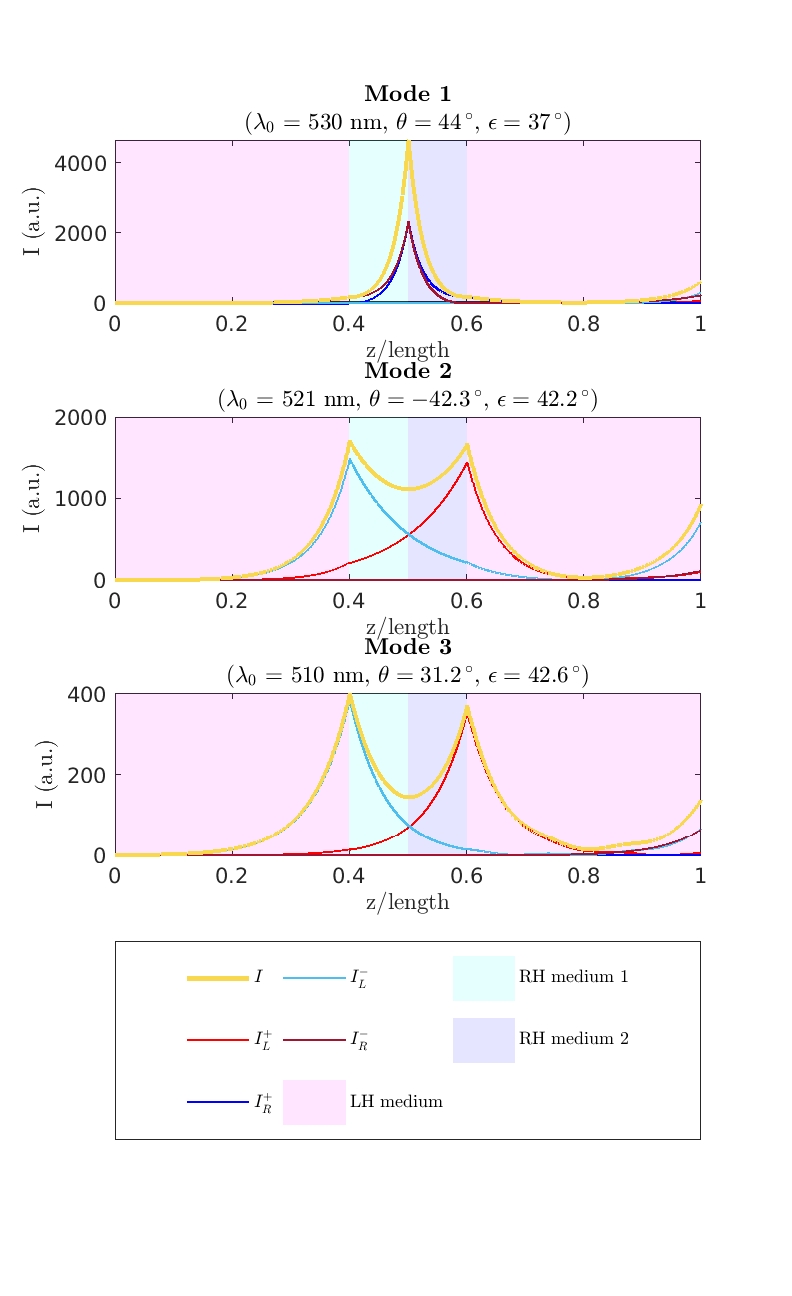
\includegraphics[width=\linewidth]{plots/hybrid_defect/pi_2/intensity_distribution}
		\caption{}
		\label{fig:hybrid_defect:intensity}
	\end{subfigure}
	\caption[Analysis of hybrid defect cavity]{Analysis of laser action for a $\frac{\pi}{2}$ defect. \ref{fig:hybrid_defect:surf} Reciprocal of the determinant of $\bm{M_{22}}$. \ref{fig:hybrid_defect:modes} Identification of output modes. \ref{fig:hybrid_defect:intensity} Intensity distribution in the cavity for found modes. The results yielded by exact theory are available in figure \ref{fig:hybrid_defect_pi2_intensity_appendix} in appendix \ref{chap:intensities}.}
	\label{fig:hybrid_defect:analysis}
\end{figure}

To study the tunability of the cavity, its output is examined over a range of defects $\psi$ going from $-\pi$ to $\pi$. The lasing loci are presented in figure \ref{fig:hybrid_defect:tuning}, showing that there seems to be a corresponding gain and defect angle allowing laser action for every detuning in the range scanned. 

Figures \ref{fig:hybrid_defect:purity}, \ref{fig:hybrid_defect:purity_lh} and \ref{fig:hybrid_defect:purity_rh} provide the distribution of output $\epsilon$ for respectively the overall 613, 465 left-handed and 148 right-handed modes found. This shows the average output $\epsilon$ is $38.66^\circ$, with a standard deviation of $3.9^\circ$. Thus, the output modes are almost pure circularly polarised. Figure \ref{fig:hybrid_defect:purity_3D} shows the distribution of modes purity against detuning and gain. Figure \ref{fig:hybrid_defect:ellipses} shows the corresponding ellipses for the extrema of the distribution of $\epsilon$.

\begin{figure}
	\centering
	\begin{subfigure}{.49\linewidth}
		\begin{subfigure}{\linewidth}
			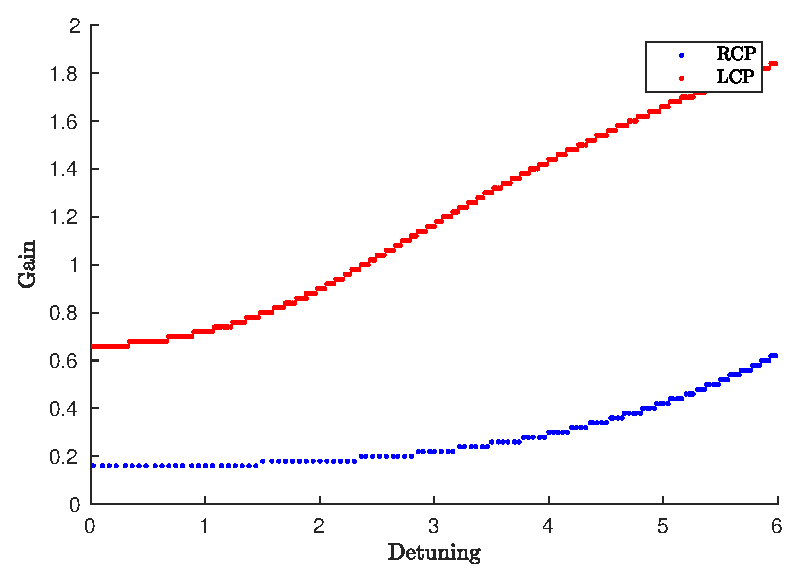
\includegraphics[width=\linewidth]{plots/hybrid_defect/tuning}
			\caption{}
			\label{fig:hybrid_defect:tuning}
		\end{subfigure}
		\begin{subfigure}{\linewidth}
			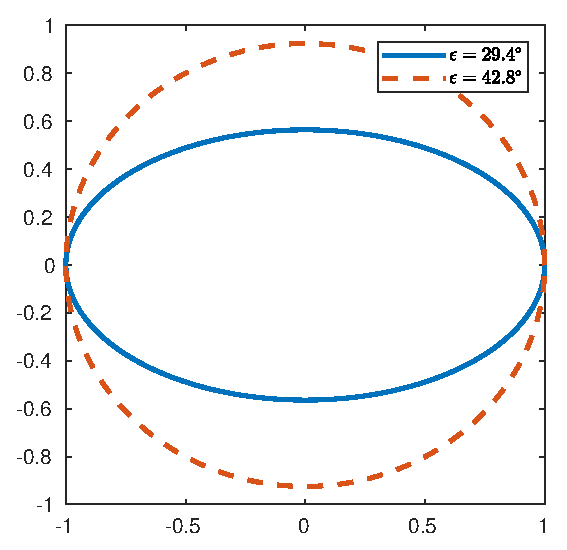
\includegraphics[width=\linewidth]{plots/hybrid_defect/ellipses}
			\caption{}
			\label{fig:hybrid_defect:ellipses}
		\end{subfigure}
		\begin{subfigure}{\linewidth}
			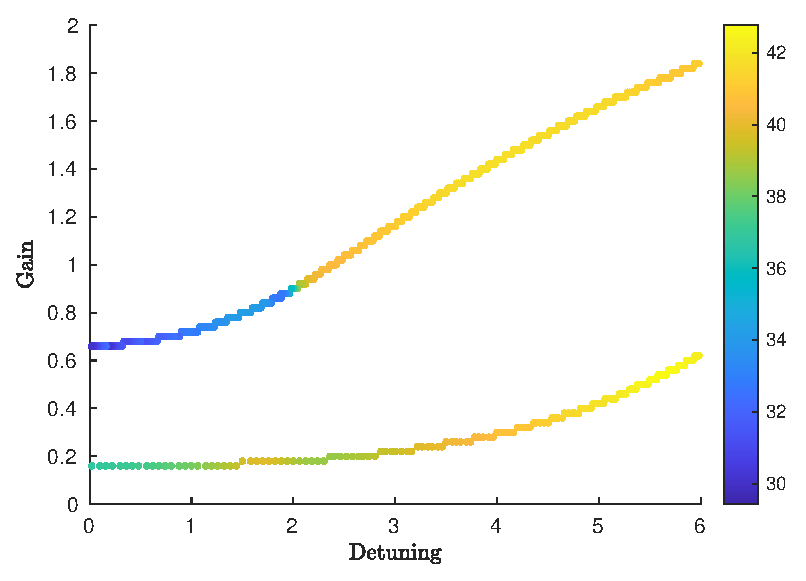
\includegraphics[width=\linewidth]{plots/hybrid_defect/purity_3D}
			\caption{}
			\label{fig:hybrid_defect:purity_3D}
		\end{subfigure}
	\end{subfigure}
	\begin{subfigure}{0.49\linewidth}
		\begin{subfigure}{\linewidth}
			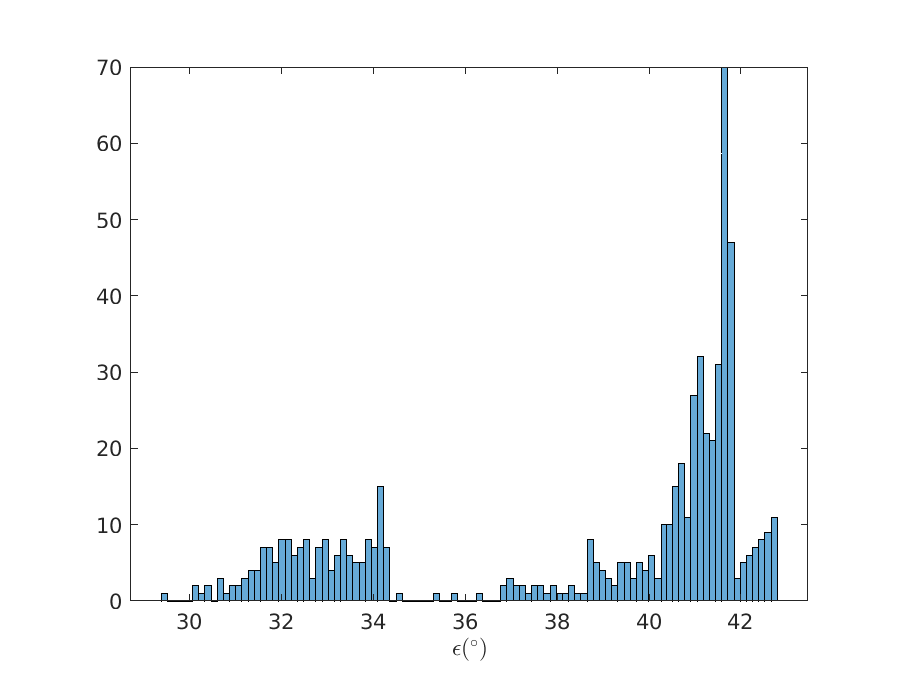
\includegraphics[width=\linewidth]{plots/hybrid_defect/purity}
			\caption{}
			\label{fig:hybrid_defect:purity}
		\end{subfigure}
		\begin{subfigure}{\linewidth}
			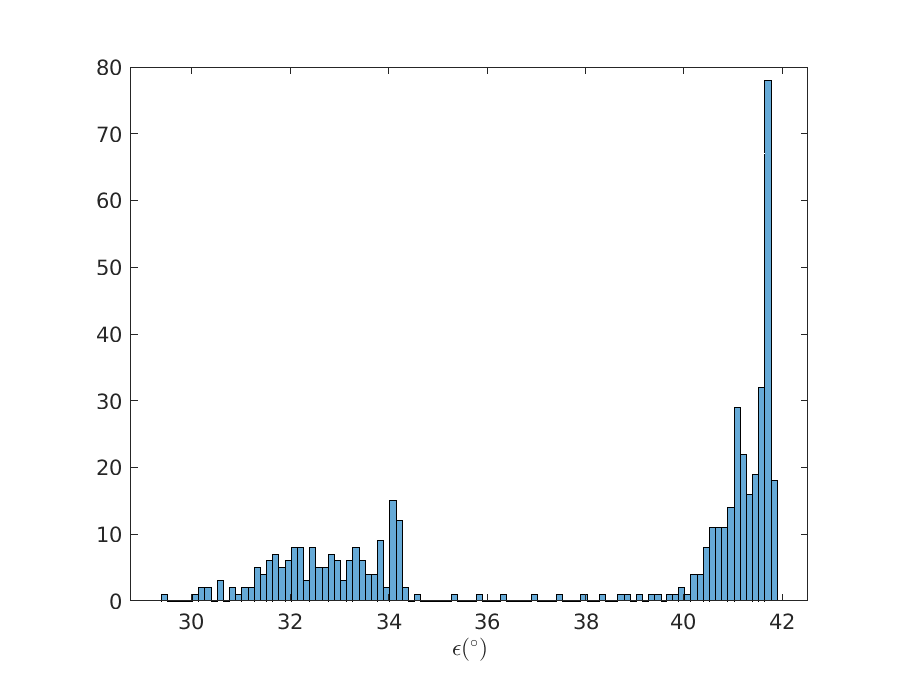
\includegraphics[width=\linewidth]{plots/hybrid_defect/purity_lh}
			\caption{}
			\label{fig:hybrid_defect:purity_lh}
		\end{subfigure}
		\begin{subfigure}{\linewidth}
			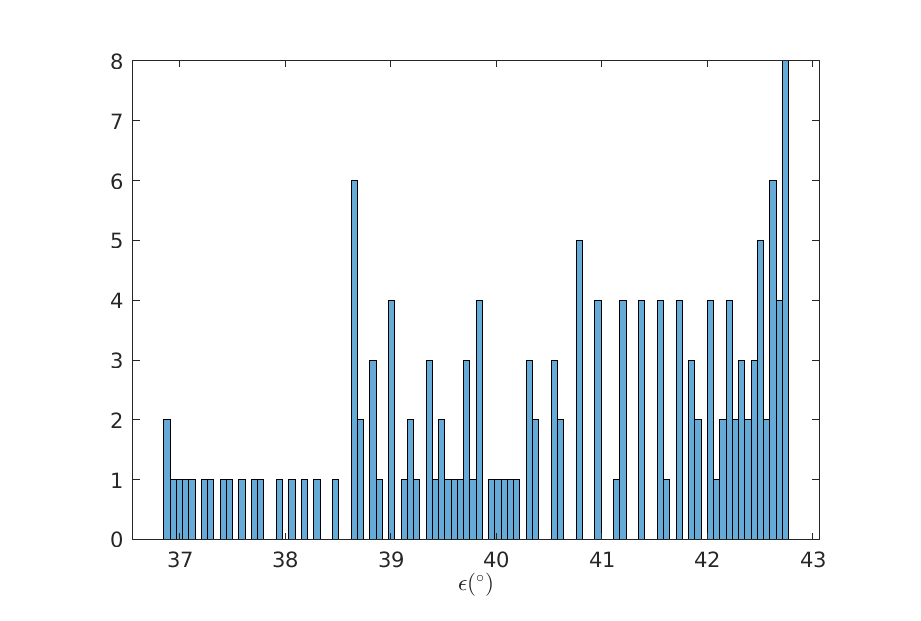
\includegraphics[width=\linewidth]{plots/hybrid_defect/purity_rh}
			\caption{}
			\label{fig:hybrid_defect:purity_rh}
		\end{subfigure}
	\end{subfigure}
	\caption[Scan through the possible defects of hybrid defect cavity]{Scan for a defect comprised in $[-\pi, \pi]$ radians. \ref{fig:hybrid_defect:tuning} Positions and handednesses of output modes. \ref{fig:hybrid_defect:ellipses} Output ellipses for the extrema of figure \ref{fig:hybrid_defect:purity}. \ref{fig:hybrid_defect:purity_3D} Distribution of $\epsilon$ for identified lasing modes. \ref{fig:hybrid_defect:purity} Distribution of output $\epsilon$ of the cavity. $\epsilon = 45^\circ$ corresponds to a perfect circle and $\epsilon=0^\circ$ to a linearly polarised output. \ref{fig:hybrid_defect:purity_lh} Distribution of output $\epsilon$ for left-handed polarisations. \ref{fig:hybrid_defect:purity_rh} Distribution of output $\epsilon$ for right-handed polarisations.}
\end{figure}

\subsection{Proposed explanation for the tunability of the cavity}

As shown in intensity distribution plots, the defect provides strong confinement of right-handed polarised light within it. Thus, this allows adjusting the effective optical length of the cavity for right-handed polarised light and, given the right gain, allows for lasing. A similar mechanism could explain tunability for left-handed polarised light. Indeed the two left-handed media also differ by a rotation corresponding to the defect. Thus, by adjusting the defect, it is possible to adjust the effective length of the cavity to a given detuning, providing laser action when the gain is suitably adjusted.

\subsection{Conclusion on hybrid defect cavity}
This design manages to combine the advantages of both defect and hybrid cavities. Indeed, it seems that it allows producing relatively pure circularly polarised modes for any detuning of the cavity, given the correct angle of defect and gain. Furthermore, for a given detuning, it seems possible to switch between left and right circularly polarised light by changing the defect and gain, which makes such a laser highly versatile. A more detailed study, perhaps analytical, aiming to give a direct way to estimate gain and angle of defect given a cavity detuning would be a great addition here.